\documentclass[aps,prd,twocolumn,superscriptaddress,amsfont,amssymb,amsmath,nofootinbib,showpacs,balancelastpage]{revtex4-1}
%\documentclass[prd,superscriptaddress,twocolumn,floatfix]{revtex4}

\usepackage{graphicx,longtable,natbib,mathrsfs,color}
\usepackage{txfonts}

\newcommand{\bs}{\boldsymbol}
\newcommand{\diff}{{\mathrm d}}
\newcommand{\Cov}{\mathsf{C}}
\newcommand{\Fish}{\mathsf{F}}
\newcommand{\Cl}{\mathcal {C}}
\newcommand{\R}{\mathcal{R}}
\newcommand{\T}{\mathcal{T}}
\newcommand{\Msun}{M_\odot}
\newcommand{\lb}{\left\langle}
\newcommand{\rb}{\right\rangle}

%
\def\apjl{Astrophys. J. Lett.}
\def\apjs{Astrophys. J. Suppl. Ser.}
\def\aj{Astron. J.}
\def\mnras{Mon. Not. R. Astron. Soc.}
\def\aap{Astron. Astrophys.}                % Astronomy and Astrophysics
\def\jcap{J. Cosmology Astropart. Phys.}
\def\aapr{Astron. Astrophys. Rev.}

\begin{document}

\addtolength{\hoffset}{-0.525cm}
\addtolength{\textwidth}{1.05cm}
\title{Reconstruction of Large Scale Structure by Nonlinear Displacement Fields}

%\author{Hao-Ran~Yu} \affiliation{}\email{haoran@cita.utoronto.ca}
%\author{Qiaoyin~Pan}
%\author{Ue-Li~Pen} \affiliation{}
%\author{Tong-Jie~Zhang} \affiliation{}
%---


%\date{Received \today; published -- 00, 0000}

\begin{abstract}
We investigate the ability of using nonlinear displacement field to reconstruct the primordial linear perturbations of the large scale structure. According to the linear Lagrangian perturbation theory, the first order primordial linear density field is given by the negative divergence of the displacement field. By running $N$-body simulations, we show that this reconstruction algorithm recovers great amount of nonlinear information in the early universe. In reality, the displacement fields can be solved from only the final stage of the density fields. This has potential to reconstruct baryonic acoustic oscillation (BAO) from current and future large scale structure surveys.
\end{abstract}

%\pacs{98.80.Es 95.36.+x}

\maketitle

\section{Introduction}\label{sec.intro}
Our universe starts from primordial Gaussian perturbations at a very early stage, and from those fluctuations, the gravitational instability drives the formation of the large scale structure (LSS) distribution of matter. These structures grow linearly until the perturbations are large enough such that first order perturbation theories are unable to analytically describe the LSS distributions. Inversely, the final stage nonlinear LSS distribution contains higher order statistics, and thus makes it more challenging to interpret the basic cosmological parameters. This leads to various attempts to recover earlier stages of LSS, in which statistics are closer to Gaussian. Because Gaussian fields can be adequately described by two-point statistics, ideally after some recovery algorithms, more information can be extracted, more straightforwardly, by power spectra or two-point correlation functions.

These algorithms include nonlinear Wiener filters in wavelet space, distribution function transforms etc. Standard BAO reconstruction algorithms smooths the nonlinear density field on linear scale ($\sim$10 Mpc$/h$) and reverse the large scale bulk flows by a negative Zel'dovich linear displacement. Here we propose a new reconstruction method that uses the nonlinear displacement field to recover the primordial density field. In the linear Lagrangian perturbation theory, the negative divergence of the the displacement field respect to Lagrangian coordinates gives the linear density field. Of course, the full displacement field is non-observable, as it requires the initial distributions of matter, however there are many techniques to estimate the nonlinear displacement field from a final distribution of matter. For example, when a homogeneous initial matter distribution is assumed, there is a unique solution of curl-less displacement field to relate the initial and final distributions without shell-crossing. This solution can be solved by a metric transformation equation \citep{1995ApJS..100..269P,1998ApJS..115...19P}. In 1-dimensional case, the solution simplifies to a reordering of matter elements by Eulerian positions, and [Hong-ming et. al.] studies this case. The homogeneous and curl-less assumptions are generally valid in cosmology [cite or proof]. Shell-crossing does exist, and this effect can be quantified by $N$-body simulations.

In this paper we track the initial and final distributions of particles in LSS $N$-body simulations, and use the displacement field to reconstruct the initial linear density field. The rest of this paper is structured as follows. In section \ref{sec.method} we describe the simulation and reconstruction algorithm. In section \ref{sec.results} we show the results of the reconstruction. Discussion and conclusion are in section \ref{sec.discussion}.

\begin{figure}[b] \centering
  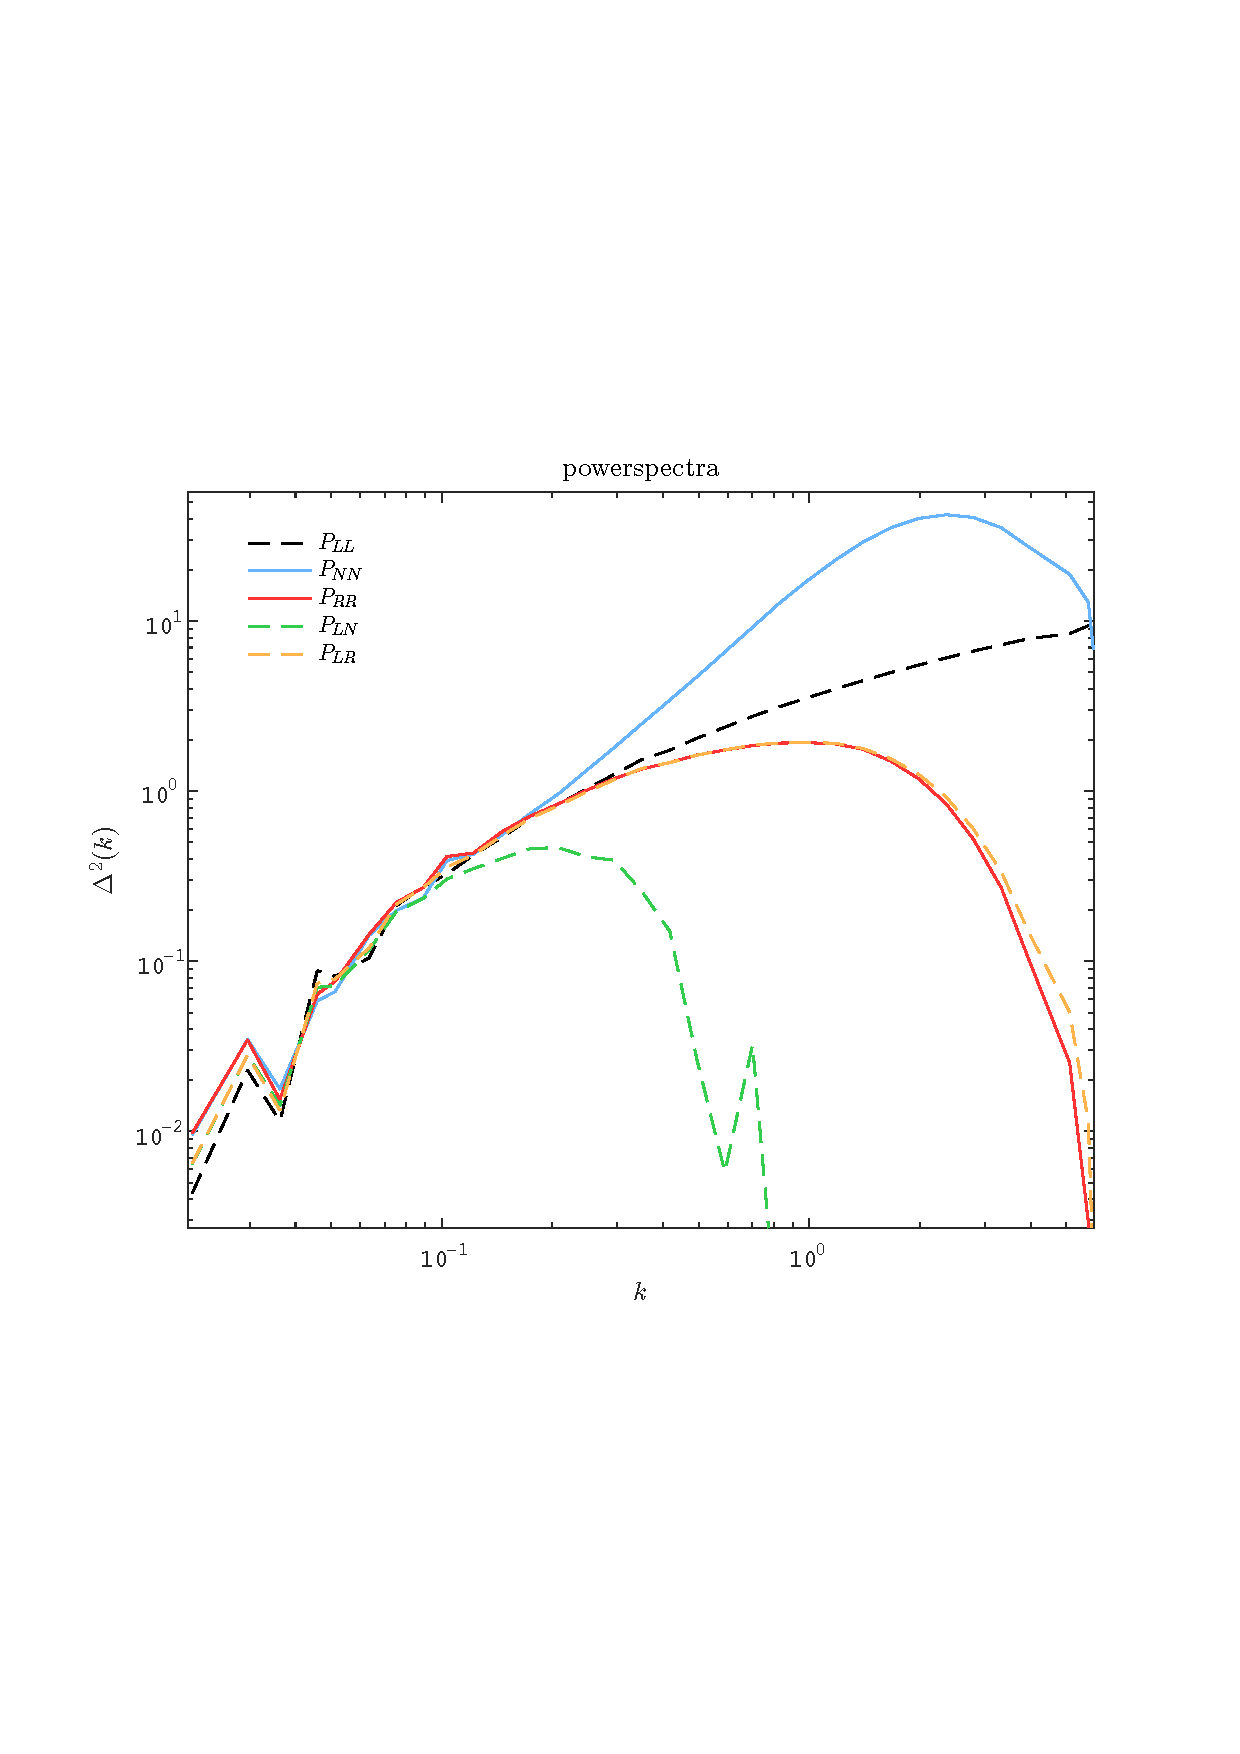
\includegraphics[width=1.0\linewidth]{fig1.pdf}
  \caption{Dimensionless auto- and cross- power spectra between nonlinear density field $\delta$, linear density field $\delta_L$ and reconstructed density field $\delta_R$.}
  \label{fig.1}
\end{figure}
\begin{figure}[t] \centering
  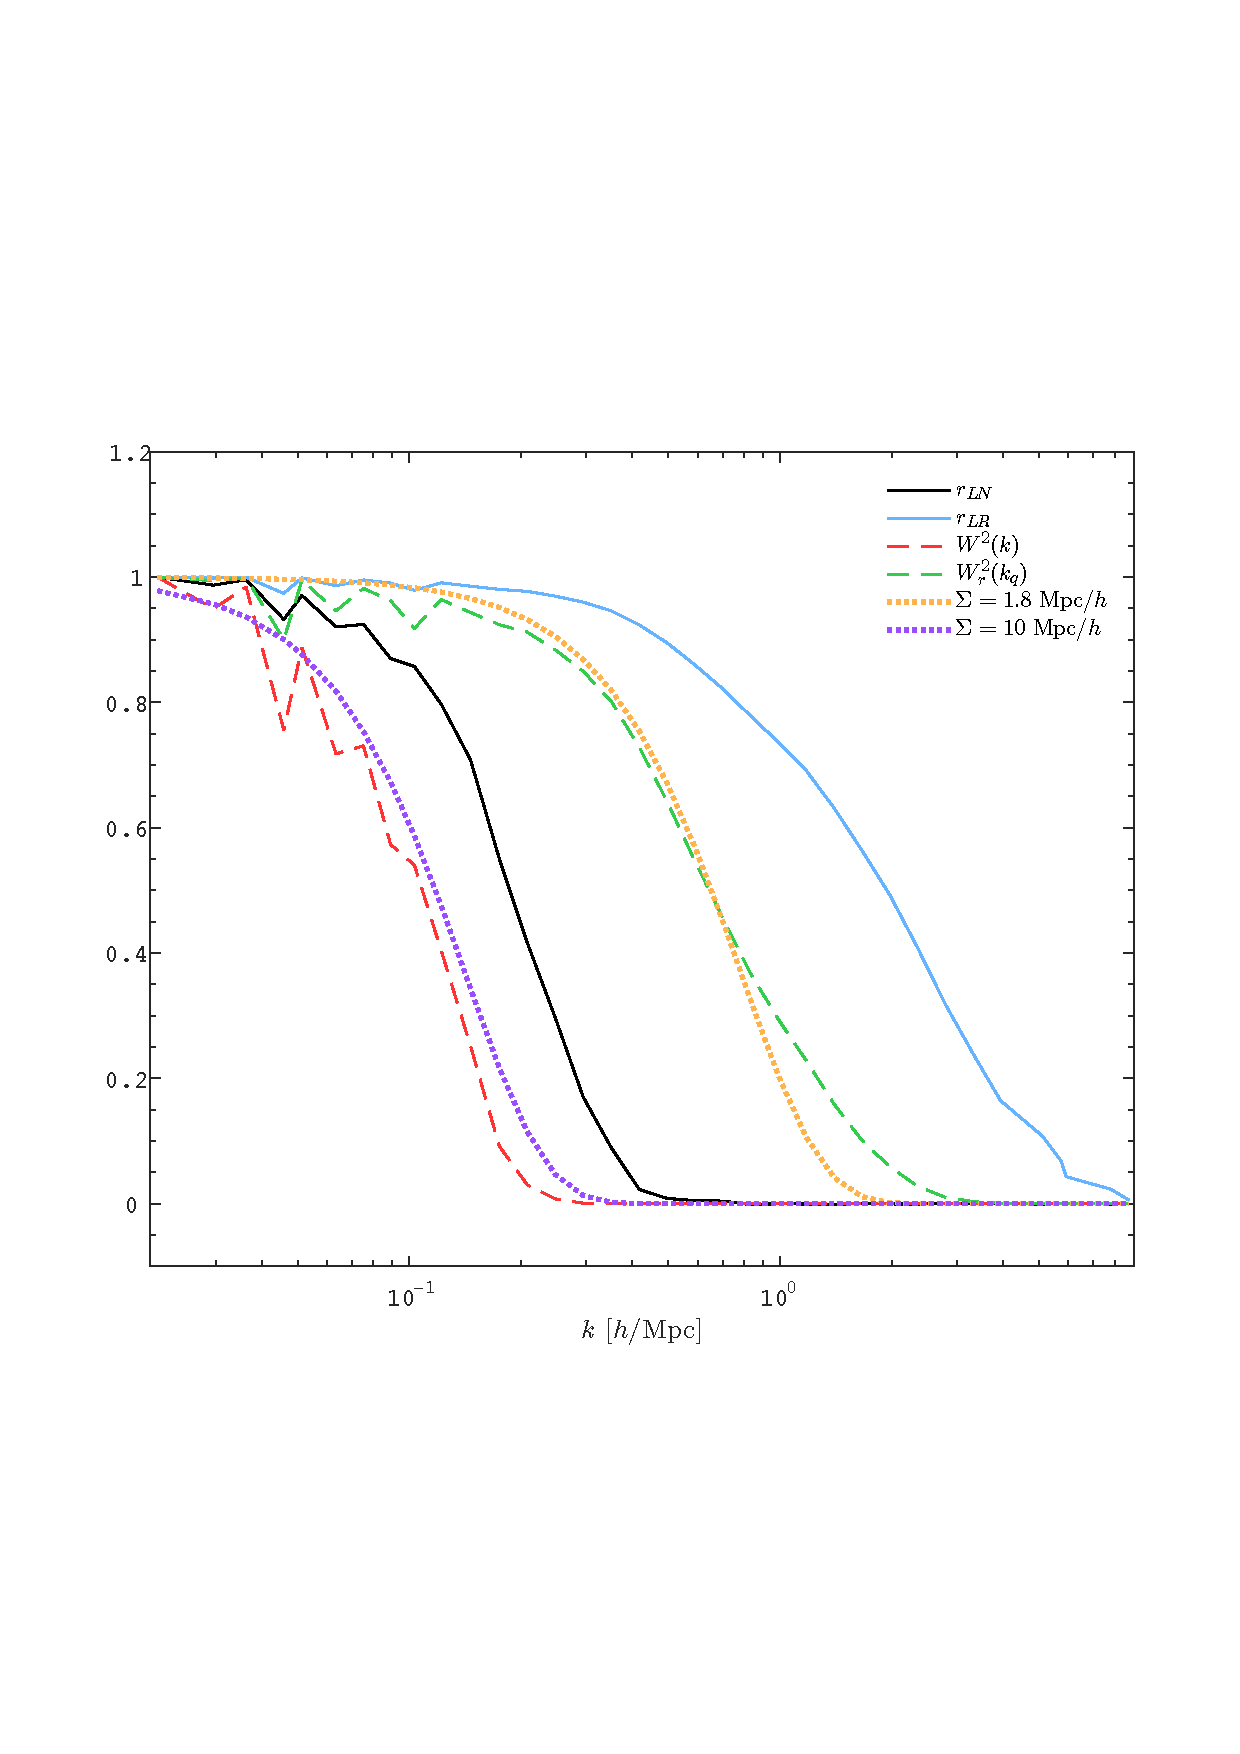
\includegraphics[width=1.0\linewidth]{fig2.pdf}
  \caption{Caption goes here.}
  \label{fig.2}
\end{figure}

\section{Method}\label{sec.method}

\subsection{Simulation}
We use the public cosmological simulation code {\tt CUBE}. Cosmological parameters are in accordance with Planck. Initial conditions are generated at redshift $z=50$ using Zel'dovich approximation. $N_p=512^3$ $N$-body particles are evolved via their mutual gravitational interactions to $z=0$, in a periodic box with $L=300$ Mpc$/h$ per side. The code is set to use standard a particle-mesh (PM) algorithm \cite{1988csup.book.....H} on a two-level mesh grids (details see \cite{2013MNRAS.436..540H}) and cloud-in-cell (CIC) is used in particle interpolations in force calculation and obtaining the density field $\rho({\bs x})$ in Eulerian coordinates ${\bs x}$ at late stages. We use density contrast $\delta\equiv\rho/\lb\rho\rb-1$ to describe the density fluctuations. The primordial linear density field $\delta_L$ is given by the initial stage and scaled to $z=0$ by the linear growth factor.

Two-point statistics of the density fields are quantified by the cross power spectrum $P_{ij}(k)\equiv(2\pi)^{-3}\langle|\delta_i(k)\delta_j(k)|\rangle$, where subscripts $i,j$ may refer to linear, nonlinear, or reconstructed density fields. When $i=j$ it reduces to the auto power spectrum $P_{ii}(k)$ or $P(k)$. We usually plot the dimensionless power spectrum $\Delta^2(k)\equiv k^3P(k)/2\pi^2$. The blue solid and black dashed curves in Fig.\ref{fig.1} show the power spectra of $\delta$ and $\delta_L$. Their difference shows the nonlinear evolution of LSS on small scales. Their cross power drops to a very low value, indicating a loss of linear information in the nonlinear power spectrum.

\subsection{Reconstruction}
In the simulation, we uses particle-ID (PID) to record the initial location ${\bs q}$ of particles, and the information is tracked until the $z=0$ and we can get the Lagrangian displacement vector ${\bs \Psi}\equiv{\bs x}-{\bs q}$ for every particle. Then these vectors are interpolated onto the initial Lagrangian coordinates ${\bs q}$ of particles and we get the displacement field ${\bs \Psi}({\bs q})$.
The raw reconstructed density field is given by the differential motion of matter elements,
\begin{equation}
    \delta_R=-\nabla\cdot{\bs \Psi}({\bs q}).
\end{equation}
In Fig.\ref{fig.1} we show the power spectrum of $\delta_R$ and its cross power with $\delta_L$. Despite of a lowered power of $\delta_R$ compared to $\delta$, it has a much higher cross power with $\delta_L$, up to a relatively smaller scale (higher $k$).


To quantify the linear information in the reconstructed density field, we decompose $\delta_R$ in Fourier space as
\begin{equation}\label{eq.decompose}
    \delta_R(k)=r'\delta_L+\delta_N,
\end{equation}
where $r'\delta_R$ is completely correlated with linear density $\delta_L$. Correlating equation (\ref{eq.decompose}) with $\delta_L$ gives
\begin{equation}
    P_{LR}=r'P_{LL}+P_{LN},
\end{equation}
where $P_{ij}\equiv\langle\delta_i\delta_j\rangle$ denotes the cross power spectrum. Since $\delta_N$ is uncorrelated with $\delta_L$, $P_{LN}=0$. With the definition of cross correlation coefficient $r\equiv P_{LR}/\sqrt{P_{LL}P_{RR}}$ and bias $b^2=P_{RR}/P_{LL}$, we solve $r'=P_{LR}/P_{LL}=rb$. We plot the cross correlation coefficient $r_{LN}$ and $r_{LR}$ in Fig.\ref{fig.2}. Clearly, $\delta_R$ contains much more linear information on smaller scales.

According to equation (\ref{eq.decompose}), the auto power spectrum is decomposed as
\begin{equation}
    P_{RR}=r^2b^2P_{LL}+P_{NN},
\end{equation}
and $P_{NN}=(1-r^2)P_{RR}$. Then we construct a Wiener filter to filter out the uncorrelated part in $\delta_R$:
\begin{equation}
    W(k)=\frac{r^2b^2P_{LL}}{r^2b^2P_{LL}+P_{NN}}=r^2.
\end{equation}
The Wiener filters are also plot in Fig.\ref{fig.2}. The estimated linear density, or the optimal reconstructed density is given by
\begin{equation}
    \tilde\delta_R=Wb^{-1}\delta_R.
\end{equation}
The full filters $Wb^{-1}$ are also plotted in Fig.\ref{fig.2}. The optimal reconstructed power spectrum is given by
\begin{equation}
    \tilde P=W^2b^{-2}P_{RR}=W^2P_{LL}+W^2b^{-2}P_{NN}.
\end{equation}
The $W^2$ describes the damping of the linear power spectrum.







\begin{figure}[t] \centering
  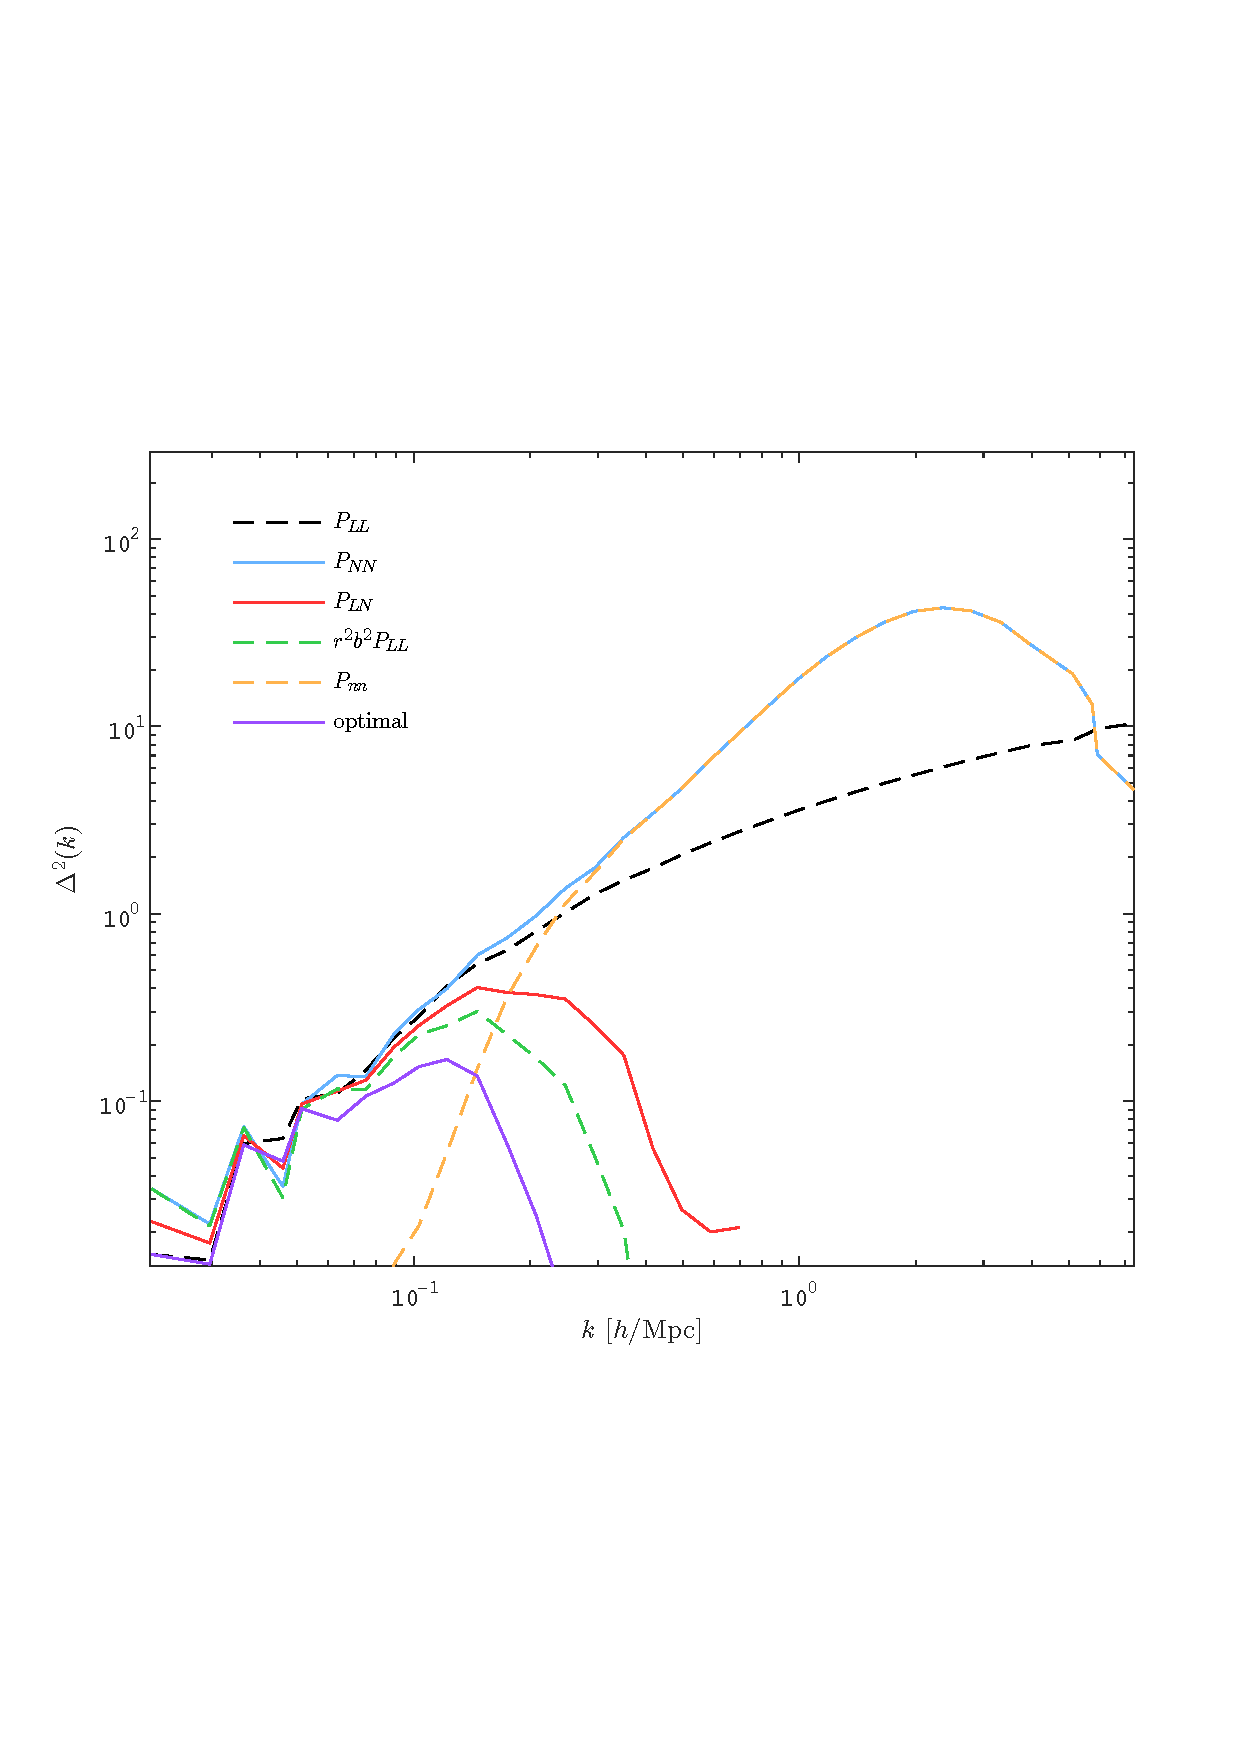
\includegraphics[width=1.0\linewidth]{fig3.pdf}
  \caption{Caption goes here.}
  \label{fig.3}
\end{figure}

\begin{figure}[t] \centering
  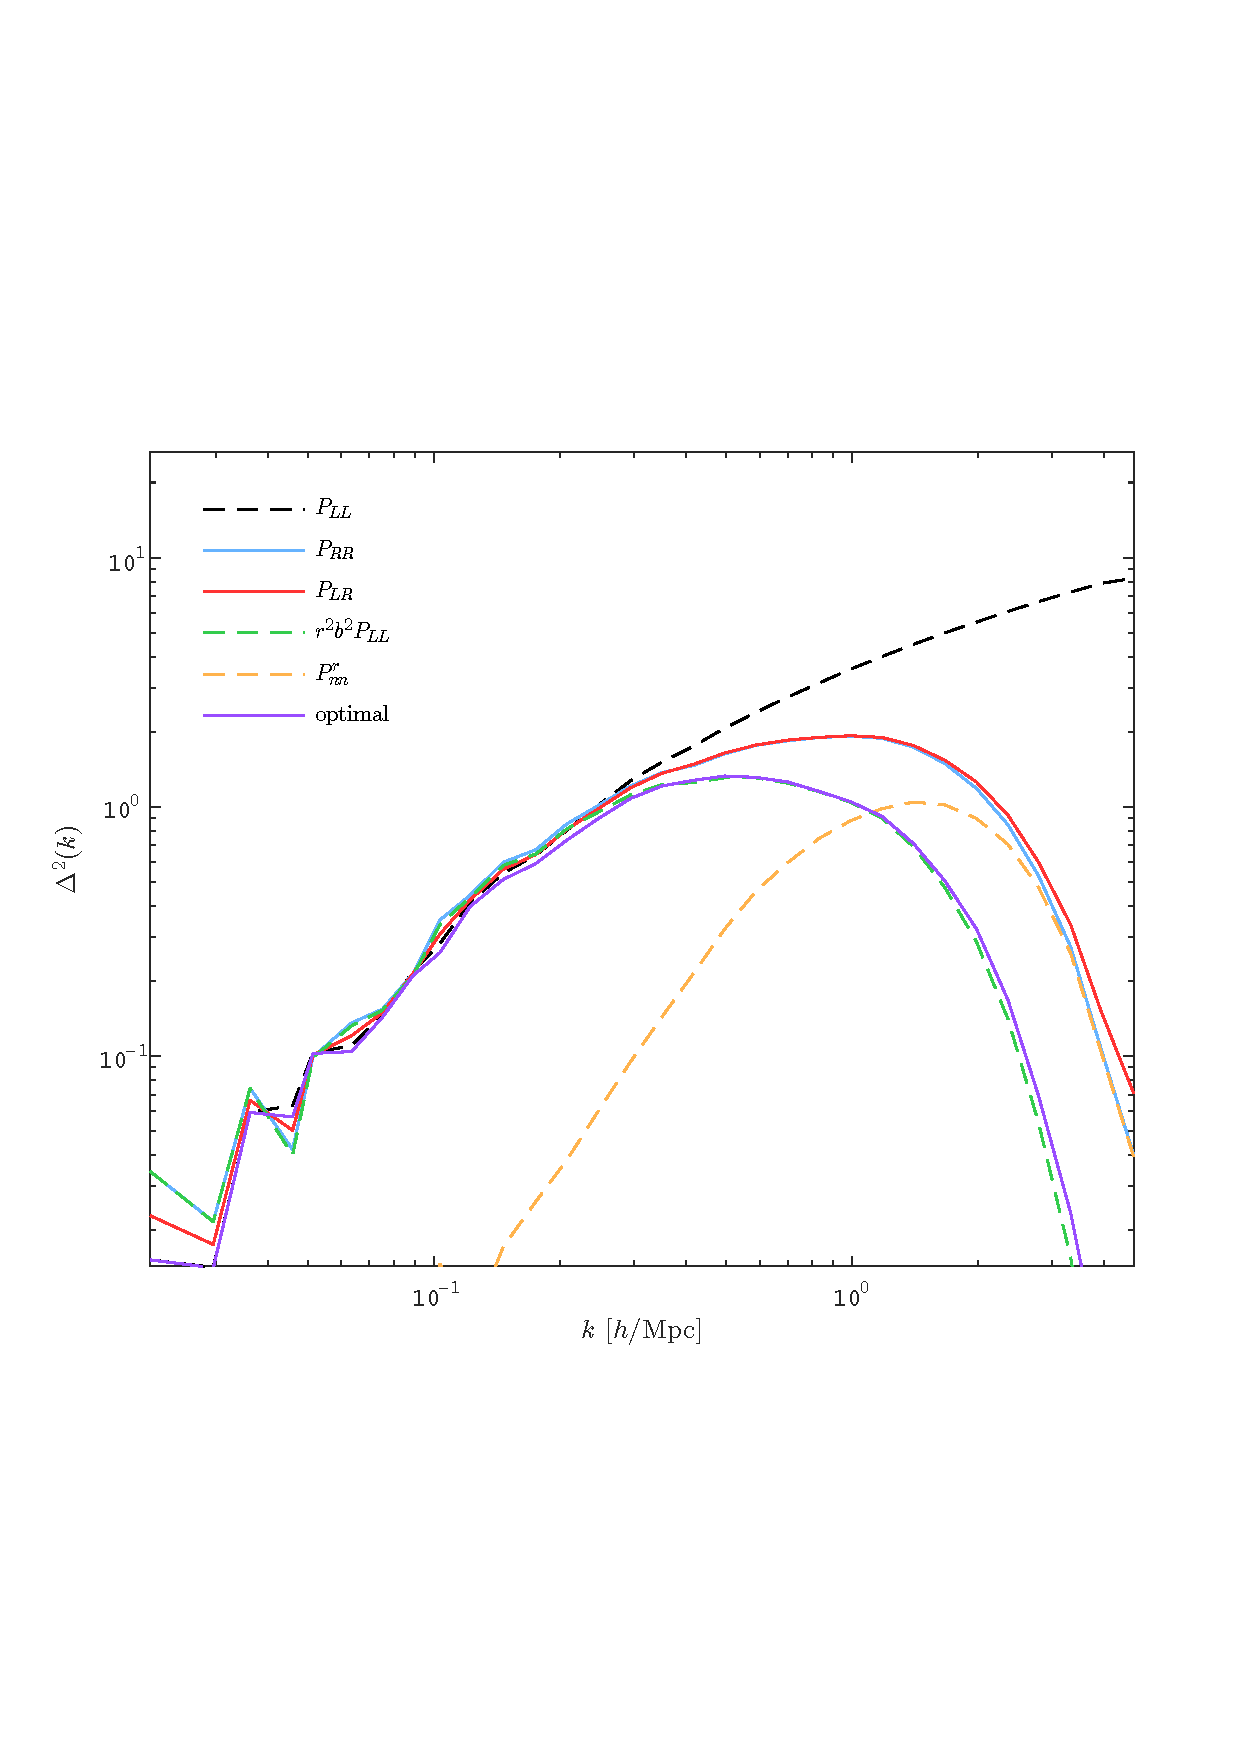
\includegraphics[width=1.0\linewidth]{fig4.pdf}
  \caption{Caption goes here.}
  \label{fig.4}
\end{figure}

\section{Results}\label{sec.results}
Fig.\ref{fig.2} shows the damping factors $W^2(k)$ for the optimal filtered nonlinear and reconstructed density fields. We fit the Gaussian BAO damping model ${\mathcal D}(k)=\exp(-k^2\Sigma^2/2)$ and give $\Sigma=1.8$ Mpc$/h$ and $\Sigma=10$ Mpc$/h$ for nonlinear and reconstructed fields.




\section{Discussion and conclusion}\label{sec.discussion}
Discussion goes here.

\section*{Acknowledgements}
Acknowledgements goes here.

%\bibliographystyle{apsrev4-1}
\bibliographystyle{h-physrev3}
\bibliography{../haoran_ref}

\end{document}
